\documentclass{jhwhw}
\author{Ian Malerich}
\title{Com S 474: Homework 3}

\usepackage{amssymb, amsfonts, mathtools, graphicx, breqn, minted, graphicx, subfig, float}
\usemintedstyle{friendly}

\DeclareMathOperator*{\argmax}{arg\,max}

\begin{document}

\raggedright

%% Problem 1
\problem{}

\begin{enumerate}
    \item Find the equation of the hyperplane (in terms of $w$) WITHOUT solving a quadratic programming problem.
	Make a sketch of the problem.
    \item Calculate the margin.
    \item Find the $\alpha$'s of the SVM for classification.
    \item Perform SVM with Matlab or R with RBF kernel and plot the result. Is this result different
	from the one you obtained by hand?
\end{enumerate}

\solution

\part
    \begin{center}
	\begin{figure}[H]
	    \centering
	    \subfloat[Original Data]{{ 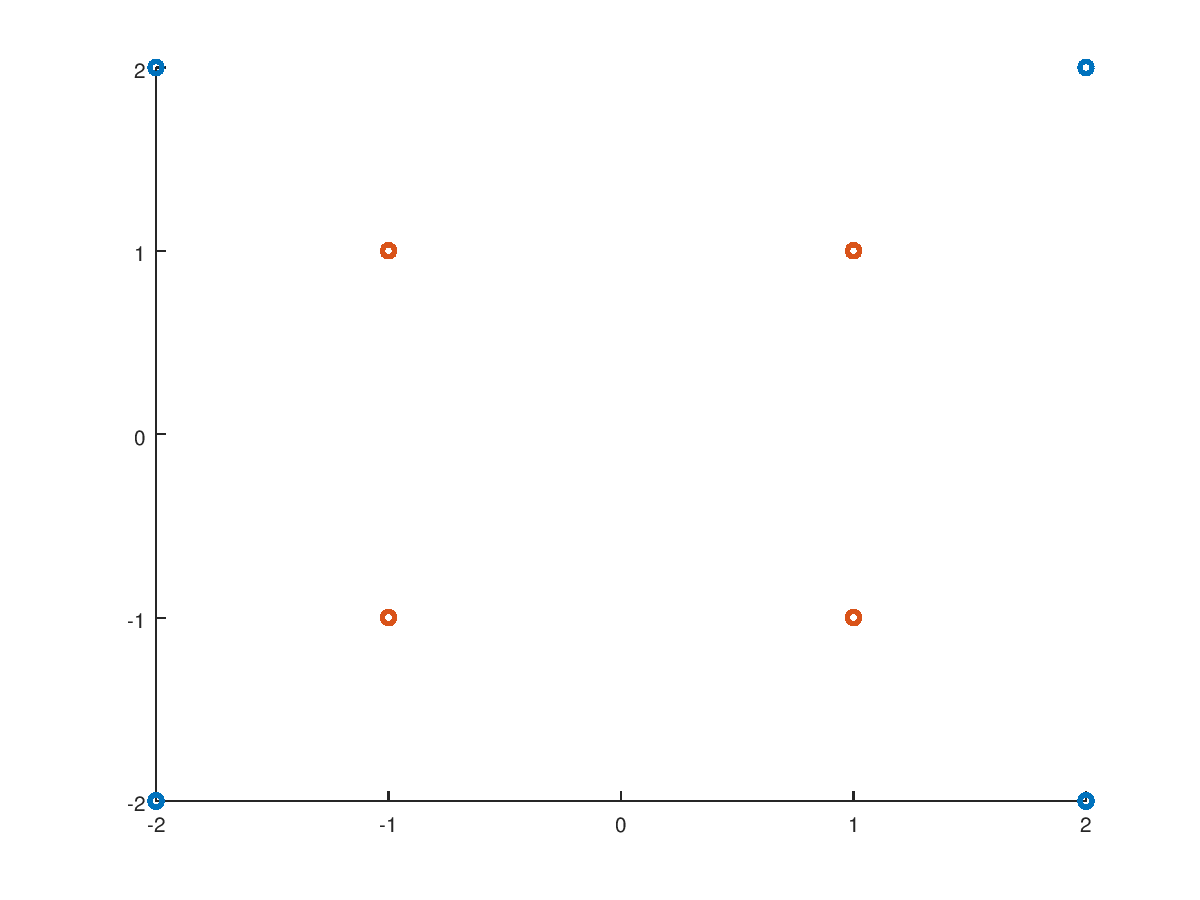
\includegraphics[scale=0.45]{data} }}
	    \subfloat[Transformed Data]{{ 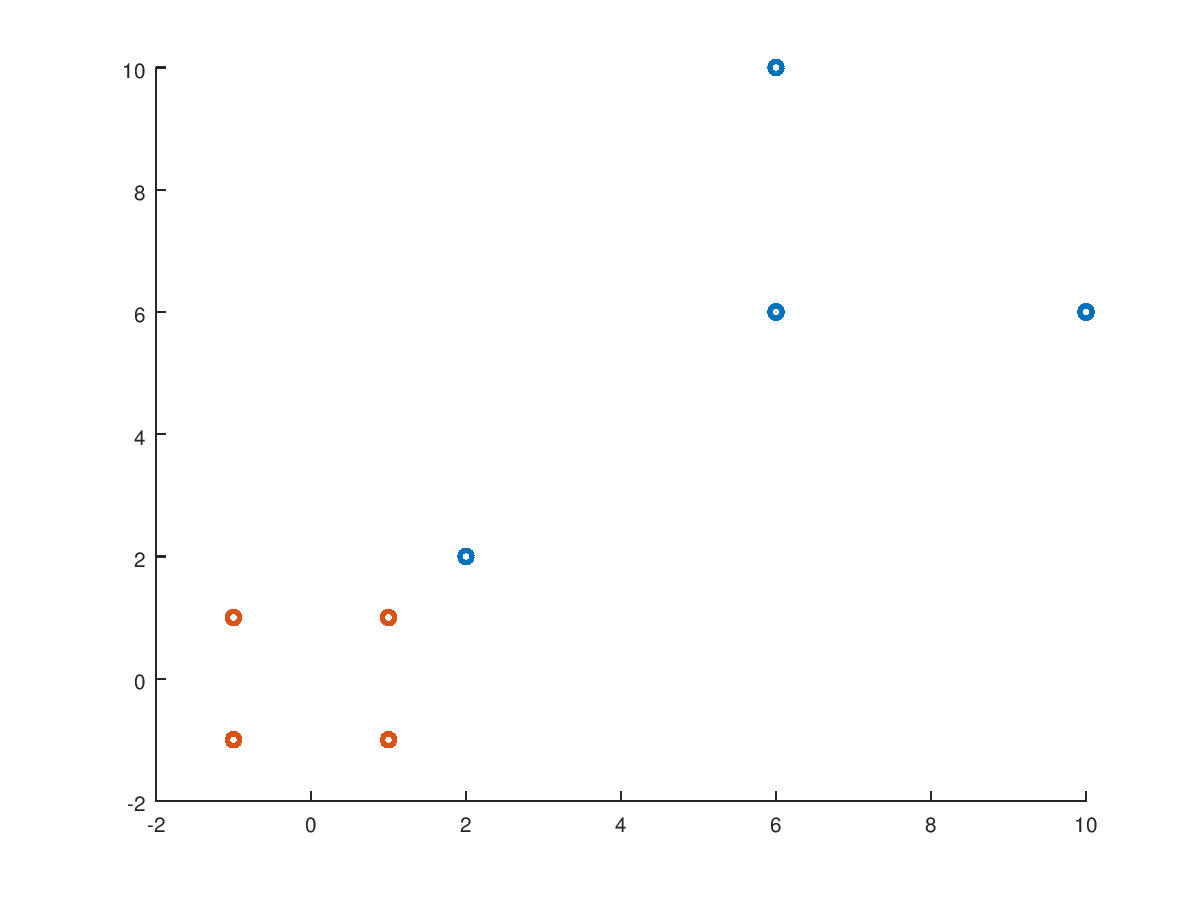
\includegraphics[scale=0.45]{transformed} }}
	\end{figure}
    \end{center}

    From this transformed data, we can clearly see our two support vectors (one for each class).
    For the orange class (-1) this is at point [1,1] and for the blue class (+1) this is at point [2,2].
    SVM requires that all points be on their respective "positive" sides of the hyperplane, thus we can
    see that this hyperplane must pass between the two support vectors we have chosen.
    This means, that if we imagine a line segment connecting connecting the points \{[1,1], [2,2]\} our
    hyperplane MUST intersect that line segment. Further, as these points are support vectors, they must lie
    at equal distance to the hyperplane, from these observations we conclude that the hyperplane will intersect
    these two points at their midpoint, this will be the point $\frac{1}{2}[1 + 2, 1 + 2] = [\frac{3}{2}, \frac{3}{2}]$. \\

    As our transformed data exists in two dimensions, our hyperplane will take the form of a line, as we know an
    intercept of this line, the only thing that remains to be found is the slope of the line, once we have that we can
    derive an equation for this line in the desired form. \\

    Intuitively we would expect the hyperplane to be perpendicular to our imaginary line segment connecting our
    two support vectors. To see why this must be the case, simply consider the case where it is not.
    At one extreme, our hyperplane is in line with both support vectors, producing a margin equal to 0, as we rotate 
    our line, this margin will increase in size. It will continue to increase in size until it reaches the perpendicular
    we are considering, if we continue to rotate beyond the perpendicular, each edge will begin to approach
    the opposite class, thus resulting in a decrease again in our margin. Thus maximum margin is achieved at the 
    perpendicular. As the line segment through \{[1,1],[2,2]\} has slope 1, this implies our hyperplane has slope -1.

    In standard form this means our line will take the form: \\
    $$
	ax + b = -1x + 3
    $$
    Some simple algebra will produce the vectorized form: \\
    \begin{align*}
	-x + 3 &= y &\\
	x + y - 3 &= 0&\\
	[1; 1]^T[x; y] - 3 &= 0 &\\
    \end{align*}
    From this we have w = [1, 1] and b = -3. \\

    To check our work we need to consider our class labels (else we would simply multiply both sides by -1),
    we expect $w'[2;2]+b = 1$ and $w'[1;1]+b = -1$. Plugging these values into matlab produces the expected results
    so I'll assume I did my work correctly.

    \begin{center}
	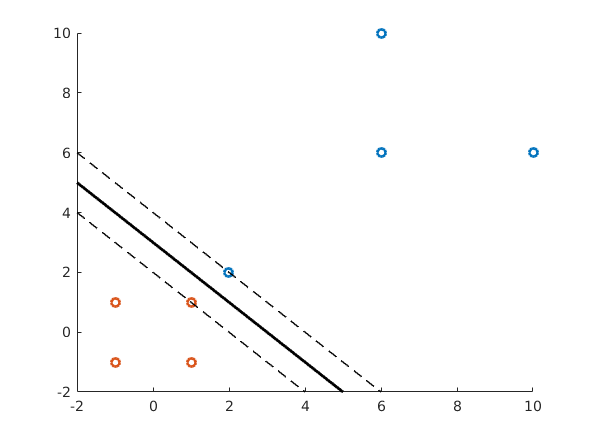
\includegraphics[scale=0.8]{boundary}
    \end{center}

    \clearpage

\part

    The margin will simply be the distance between my two support vectors.

    \begin{align*}
	dist([1, 1], [2, 2]) &= sqrt((2 - 1)^2 + (2 - 1)^2) &\\
	&= sqrt(2(1)^2) &\\
	&= sqrt(2) &\\
    \end{align*}

    Thus we find we have a margin of $sqrt(2)$.

\part

    Note that the majority of our points are not support vectors, for all of these points we have that 
    $\alpha = 0$. Note that our support vectors are observation 1 and 5, thus we still need to find
    $\alpha_1$ and $\alpha_5$. 
    From my notes we have that 
    $ w^\intercal = \Sigma_{i=1}^{m}\alpha_i Y_i x_i^\intercal$, noting that each class only has 
    one support vector we can simplify this as follows
    $$
	w^\intercal = \alpha_1 * [2; 2]^\intercal + -\alpha_5 * [1; 1]^\intercal
    $$
    This is a 2x2 linear system, format it as such.
    $$
	\begin{bmatrix}
	    1 \\ 1
	\end{bmatrix}
	= 
	\begin{bmatrix}
	    2 & -1 \\
	    2 & -1 \\
	\end{bmatrix}
	\begin{bmatrix}
	    \alpha_1 \\
	    \alpha_5
	\end{bmatrix}
    $$
    From here it is pretty obvious that $\alpha_5 = \alpha_1$ denote this $\delta$
    and we have $1 = 2\delta - 1\delta = (2 - 1)\delta = \delta$.
    Thus $\delta = 1$.

    \begin{align*}
	\alpha_1 &= 1 &\\
	\alpha_5 &= 1 &\\
	\alpha_i &= 0 $ otherwise$ &\\
    \end{align*}

\part

    \begin{center}
	\begin{figure}[H]
	    \centering
	    \subfloat[By Hand]{{ 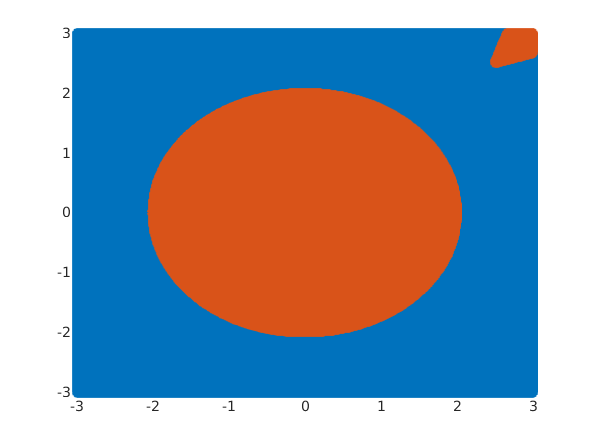
\includegraphics[scale=0.6]{p1predict} }}
	    \subfloat[Matlab]{{ 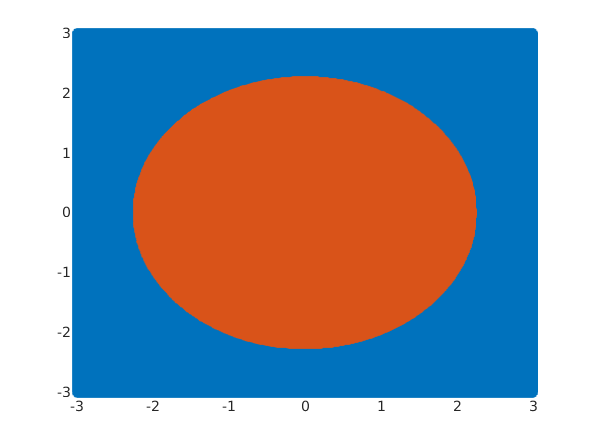
\includegraphics[scale=0.6]{predict} }}
	\end{figure}
    \end{center}

    As shown in the figure the classifier computed by hand appears to misclassify points in the top right corner,
    I only had time to to check each classifier within the bounds [-3,3] on each axis, so I don't know if this trend
    would continue if a larger bound was used. By performing some simple arithmetic (see code below), given a
    $\deltap$-step of 0.005 over the given bounds, the hand written classifier disagreed with matlabs svm
    classifier 7.772\% of the time. \\

    Despite this difference, the results performed by hand are very close to the result produced by matlab. \\

    \clearpage
    \inputminted[frame=lines,framesep=2mm]{matlab}{p1.m}
    \inputminted[frame=lines,framesep=2mm]{matlab}{phi.m}
    \inputminted[frame=lines,framesep=2mm]{matlab}{p1predict.m}

%% Problem 2
\problem{}

    Verify by means of simulation that each bootstrap sample will contain 1 - 1/e $\approx$ 63.2 of the original sample.

\solution

    \begin{center}
	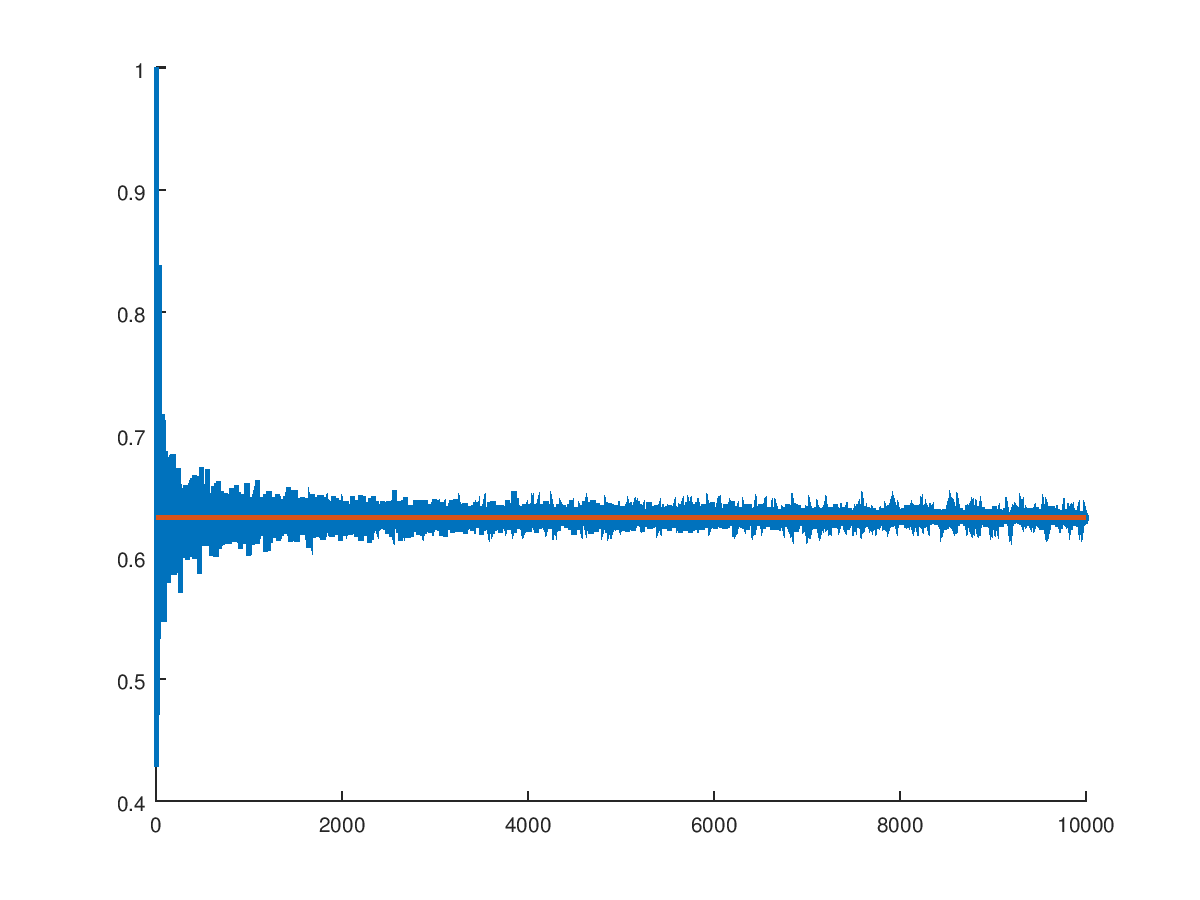
\includegraphics[scale=0.8]{p2.png}
    \end{center}

    The graph mostly speaks for itself, the orange line denotes 1 - 1/e, and the blue denotes each
    iteration of bootstrapping. As the number of iterations increases, the percentage the bootstrap contains
    of the original sample approaches the orange line (1 - 1/e). Even at 10000 iterations there appears to be
    an impact of the random values, I would imagine as we continued to increase the number of iterations
    this would taper off significantly. \\

    Again, code is provided below. \\
    \clearpage
    \inputminted[frame=lines,framesep=2mm]{matlab}{p2.m}

%% Problem 3
\problem{}

    Compare SVM and LS-SVM on the ozon level detection data set on Blackboard.
    This dataset contains 72 measurement variables and was measured between 1/1/1998 and 12/31/2004.
    All missing values have been removed. The goal is to detect whether there was too much ozon (class label 0)
    or a normal day (class label 1). The class label is the last variable. Set up the simulation and clearly describe what
    you are doing and why. Finally, state, according to your findings (boxplots, ROC curves, etc.), the best
    classifier for this problem.

\solution

    I ran svm and lssvm using the available kernel functions, then for each run usdross validation
    to estimate the misclassification rate. In general, svm took much longer than lssvm, and I could not
    get matlab to use the polynomial kernel on the data at all (see comments for full details).
    The best result produced via svm was via the rbf kernenl, which had a misclassification rate of 6.71\% and took
    148.5 seconds. In contrast each kernel worked for lssvm and took roughly half as long as their svm counterparts.
    The linear kernel of lssvm performed worse than any of the the linear and rbf kernels of svm, but the rbf
    kernel for lssvm performed the best out of all options I tested with a misclassification rate of 5.96\%.
    In terms of computation time, rbf-lssvm was slower than other lssvm kernels, but still plenty fast compared
    to the svm kernels (taking 75.9 seconds). \\
    \bigbreak
    Seeing as the rbf kernel seemed to be performing best for both, I generated a box plot to get a closer look at their 
    performance. For sake of computation time, these were found by using a random subset of 500 samples for each
    of my 100 iterations (0.75/0.25 training/test split, see code for details). With the exception of where
    they were lucky enough to have roughly 0\% misclassification error, we can clearly see from the box plot that
    lssvm consistently performs better than the svm classifier.

    \begin{center}
	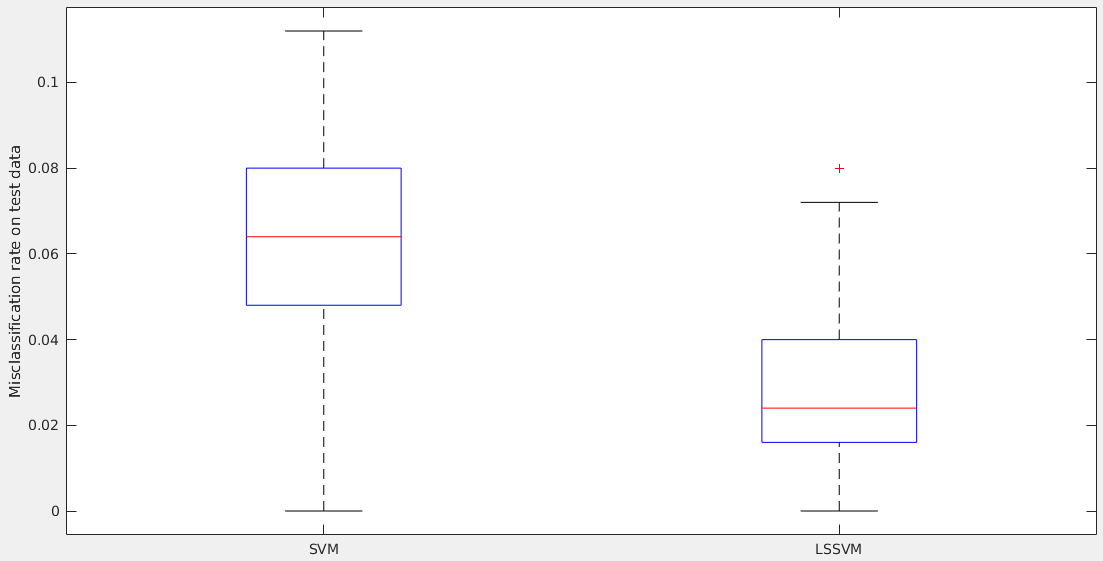
\includegraphics[scale=0.4]{p3_boxplot.png}
    \end{center}

    \inputminted[frame=lines,framesep=2mm]{matlab}{p3.m}

\end{document}
